\documentclass[11pt]{report}
%\usepackage[german]{babel}

%(Rust) Code Snippets
\usepackage{minted}
\usemintedstyle{borland}

\setminted{
framesep=2mm,
fontsize=\footnotesize,
linenos
}
%\usemintedstyle{trac}

%table cells
\usepackage{makecell}

%chapter style
\usepackage{titlesec}
\titleformat{\chapter}{\normalfont\huge\textbf}{\thechapter.}{20pt}{\huge\textbf}


%Graphs
\usepackage{pgfplots}
\pgfplotsset{width=15cm,height=7.5cm,compat=1.9}
\usepgfplotslibrary{external}
\tikzexternalize

%Definitions
\usepackage{amsthm}
\usepackage{mdframed}

\NewDocumentCommand\newmdtheoremenvnonumber{O{} m m }{%
  \newtheorem*{#2}{#3}
  \BeforeBeginEnvironment{#2}{%
     \begin{mdframed}[#1]}%
  \AfterEndEnvironment{#2}{%
     \end{mdframed}}%
}

\newmdtheoremenvnonumber{mydefinner}{\mydeflabel}
\newcommand{\mydeflabel}{}
\newenvironment{mydef}[1]
 {\renewcommand\mydeflabel{#1}\begin{mydefinner}}
 {\end{mydefinner}}

\newcommand{\attribution}[1]{\textup{(#1)}}



%Citations
\usepackage[style=authoryear, backend=bibtex, urldate=long, sorting=none, defernumbers=true,autocite=superscript]{biblatex}
\addbibresource{refs.bib}
\usepackage{csquotes}


%Math Library
\usepackage{amsmath}

%Images Library
\usepackage{float}
\usepackage{graphicx}
\graphicspath{ {./images/} }

%General Layout
\usepackage{geometry}
\geometry{
    a4paper,
    left=20mm,
    right=20mm,
    top=30mm,
    bottom=30mm,
%    total={6in, 8in}
}

%Background image
\usepackage[pages=some]{background}

%Liks of TOC
\usepackage{hyperref}
\usepackage{lstmisc}
\usepackage{holtxdoc}
\usepackage{pgfregressiontest}
\usepackage{hhline}

\hypersetup{
    colorlinks,
    linkcolor={blue!50!black},
    citecolor={blue!50!black},
    urlcolor={blue!80!black}
}


\backgroundsetup{
scale=1,
color=black,
opacity=1,
angle=0,
contents={%
\hspace*{13.5cm}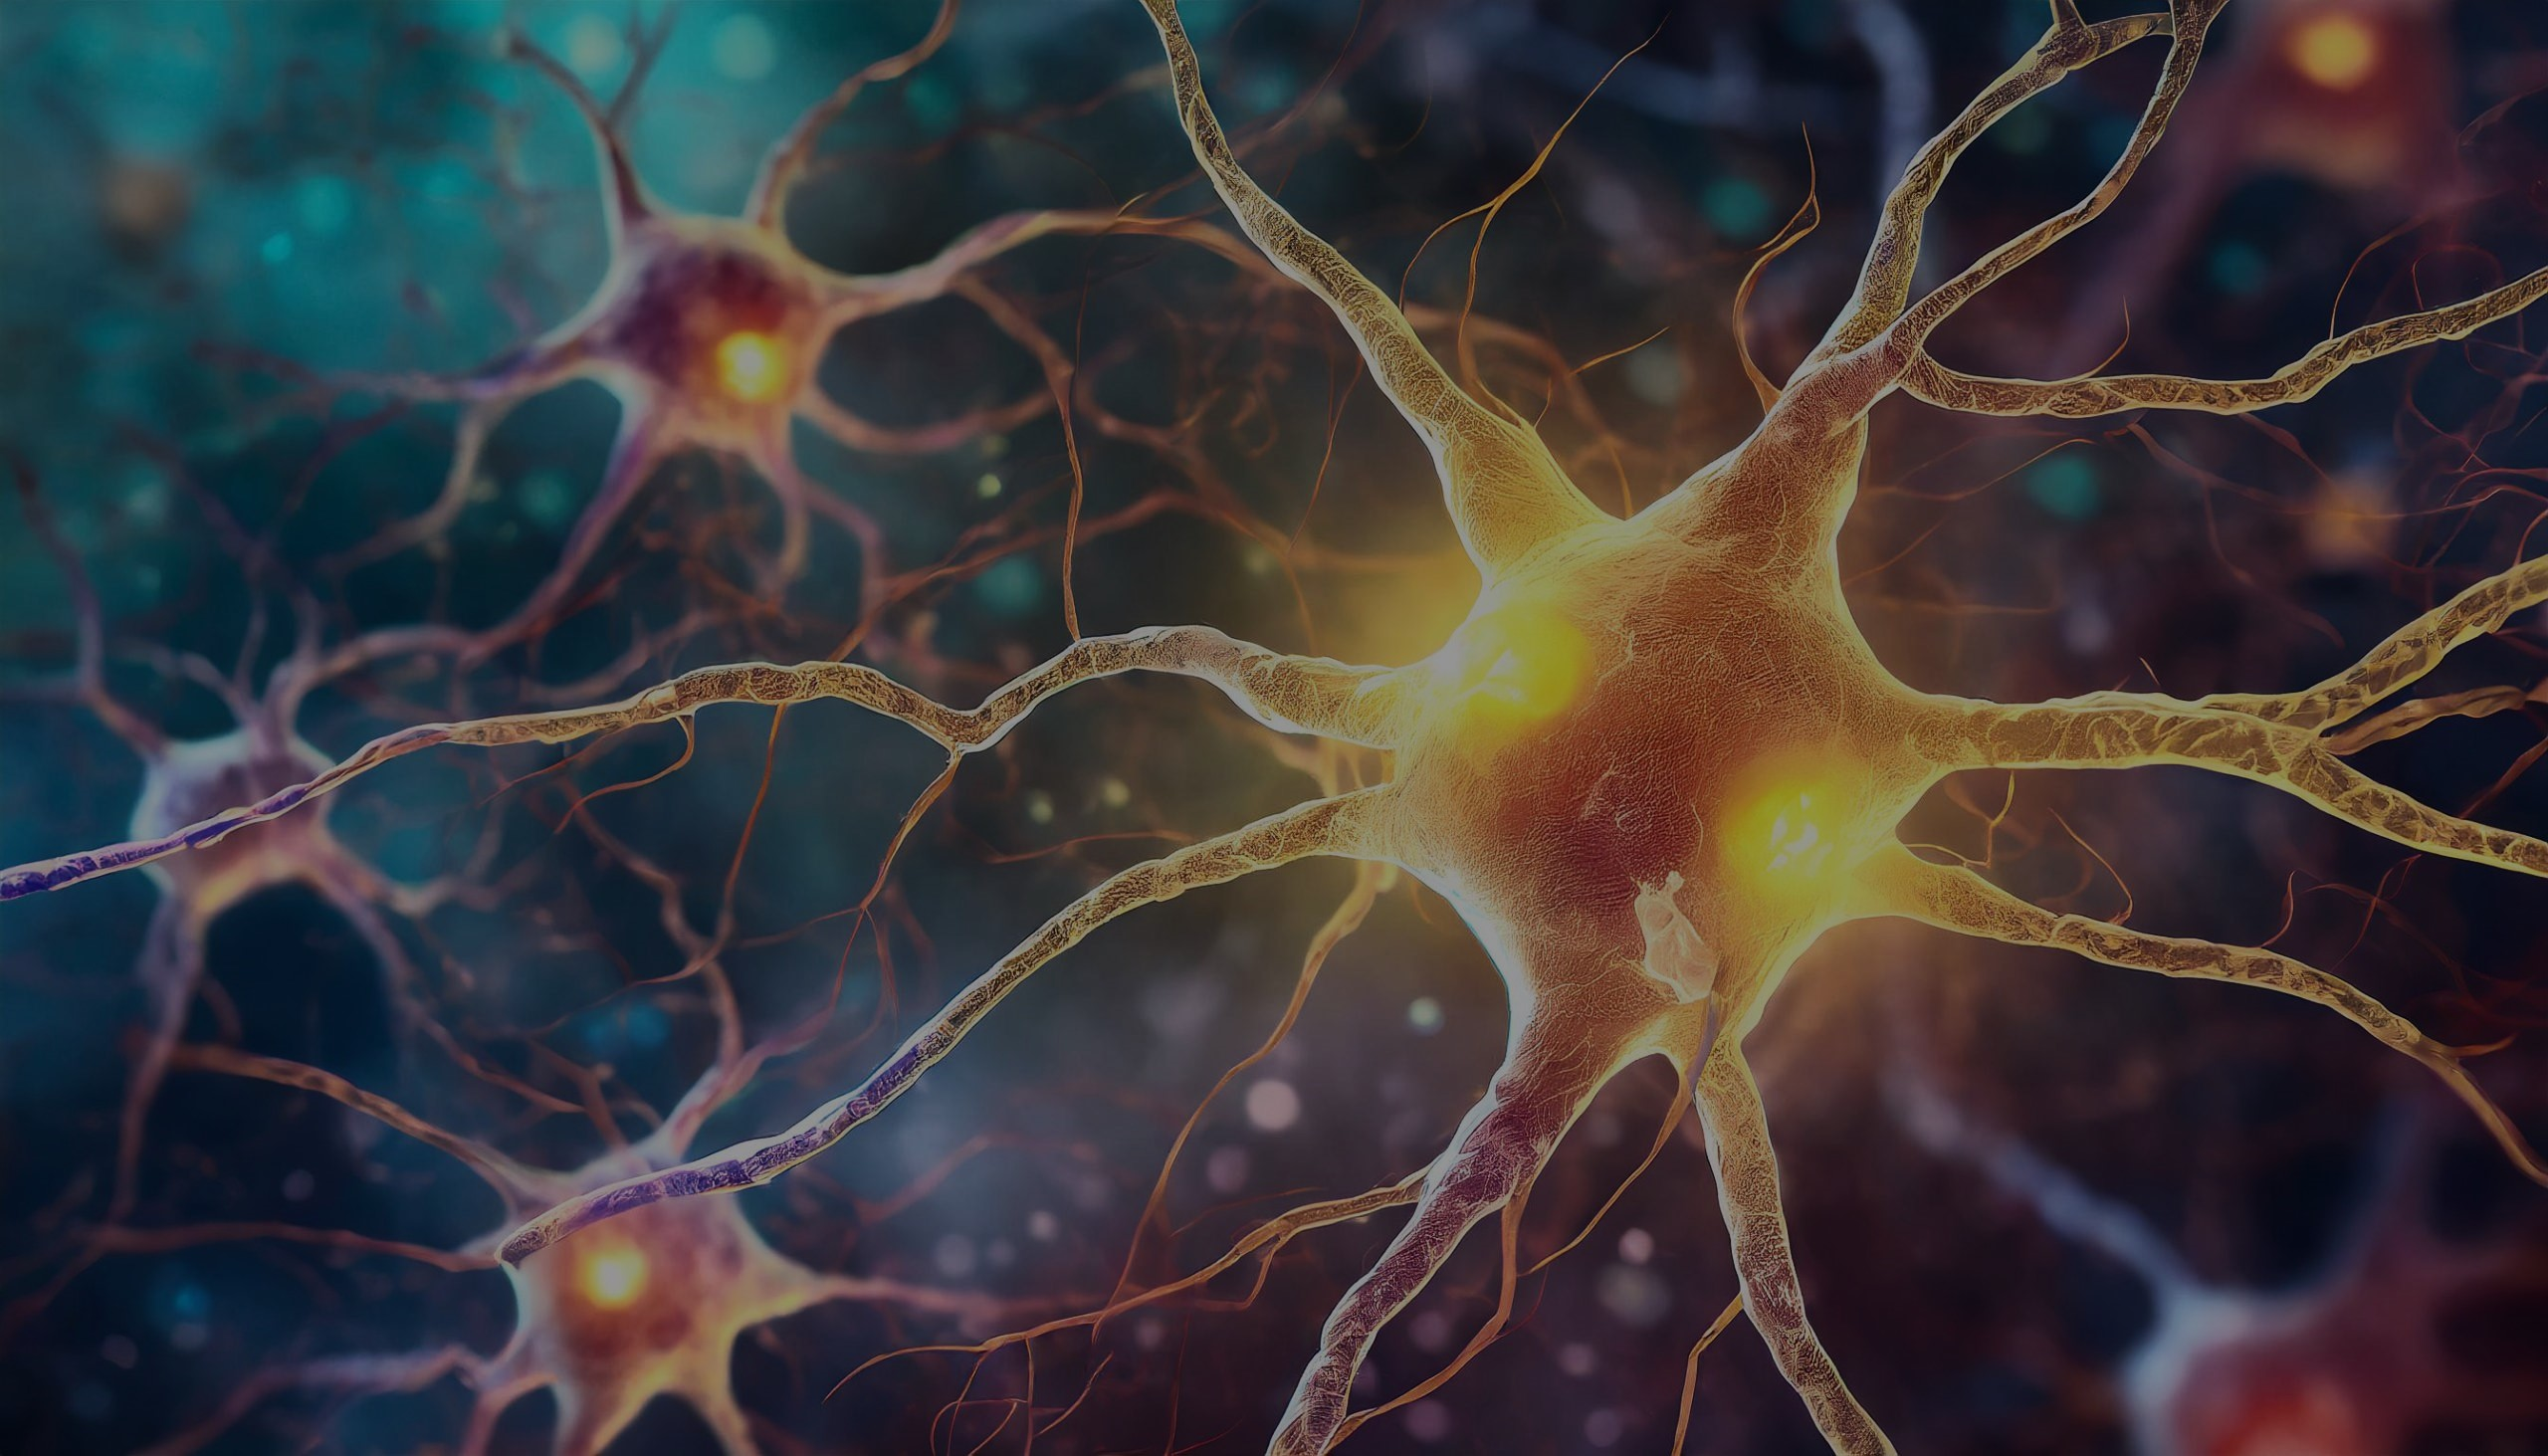
\includegraphics[width=3\paperwidth,height=\paperheight]{abstract_neurons3}
  }%
}


\begin{document}
    \pagenumbering{gobble}
    \begin{titlepage}
        \BgThispage
            \color{white} {
                \begin{center}
                    \Large \textsc{Matura Thesis}\\Kantonsschule Hohe Promenade\\
                    \rule[0.1cm]{15.8cm}{0.1mm}\\
                    \vspace{3cm}
                    \Huge \textbf{ \textsc{How can you develop \\Evolutionary Neural Networks which \\learn to play Board Games?}}\\
                    \vspace{0.8cm}
                    \Large \textit {Implementation and Study of\\ Evolutionary Neural Networks inspired\\ by the NEAT Algorithm}\\
                \end{center}
                \vspace{3cm}
                \rule[0.1cm]{15.8cm}{0.1mm}\\
                \vspace{9cm}\\
                \begin{minipage}[t]{0.47\textwidth}
                \large\textbf {Thesis By:}\\
                \end{minipage}
                \hfill
                \begin{minipage}[t]{0.47\textwidth}\raggedleft
                \large\textbf {Lucien Kissling 6e}\\
                \end{minipage}
                \begin{minipage}[t]{0.47\textwidth}
                \large \textbf {Year:}\\
                \end{minipage}
                \hfill
                \begin{minipage}[t]{0.47\textwidth}\raggedleft
                \large \textbf {2025}\\
                \end{minipage}
                \begin{minipage}[t]{0.47\textwidth}
                \large \textbf {Supervisor:}\\
                \end{minipage}
                \hfill
                \begin{minipage}[t]{0.47\textwidth}\raggedleft
                \large \textbf {Timo Schenk}\\
                \end{minipage}
                \begin{minipage}[t]{0.47\textwidth}
                \large \textbf {Co Examiner:}\\
                \end{minipage}
                \hfill
                \begin{minipage}[t]{0.47\textwidth}\raggedleft
                \large \textbf {Dr. Arno Liegmann}\\
                \end{minipage}
                \vfill
            }
        \clearpage
    \end{titlepage}
    \pagenumbering{arabic}
    \setcounter{page}{2}
    \tableofcontents
    \chapter{Introduction}\label{ch:introduction}
    \section{Preface}\label{sec:preface}
    Ever since I got into Computer Science a few years ago, I was fascinated by the Idea of Algorithms that solved various Problems.
    Therefore, I participated in the SOI (Swiss Olympiad in Informatics) where we were taught everything about developing and programming Algorithms and their Data Structures.
    \\ \\
    In recent years although, a new field of Computer Science has gained a lot of attention, where those Algorithms are not programmed by humans, but evolved by a computer.
    This field called Machine Learning immediately got my excitement and two years ago a friend of mine and I had our first practical experience with it.
    We developed a simple Neural Network, which helped us predict the color of a lego brick in front of a color sensor based on the RGB values in various lighting conditions.
    \\ \\
    A Neural Network (NN) forms the basis of most Machine Learning Models and I will therefore explain it in much detail in the following Chapters.
    In simple terms, a NN is a strongly simplified artificial model of the human brain as a NN consists of an interconnected web of Neurons through which information flows and gets computed.
    \\ \\
    Although the NN we developed two years ago already learned on its self, we still had to provide data for it to learn from.
    This meant that we had to manually scan the RGB values of the lego bricks and then label them with the color they represented.
    The aim of my Matura Thesis therefore is to take the idea of self learning a step further by developing Neural Networks, which don't need this kind of data with solutions predefined by humans.

        \section{Thesis Statement}\label{sec:thesis-statement}
    As mentioned in the previous Section, this Thesis will explore the field of Neural Networks (NNs) that learn without data provided by humans, which is called unsupervised learning.
    The solution this Thesis will focus on are Evolutionary Neural Networks (ENNs), a combination of Neural Networks and Genetic Algorithms.
    \\ \\
    In this Thesis, I develop my own simplified implementation ENNs and then train them on some Board Games.
    The research effort consists of testing the ENN algorithm with different Parameters and Features to see how well it can learn to play the games in different configurations.
    My approach also draws inspiration from the NEAT Algorithm developed by Kenneth O. Stanley and Risto Miikkulainen in 2002, where the NNs start minimally in the first generation and then develop complexity over time.\footcite[p.105-106]{Neat_02}
    The first game I will train the ENNs on is Nim, a simple game where two players take turns removing matches from different stacks.
    \\ \\
    In specific, this Thesis aims to answer following questions:
    \begin{itemize}
        \item How can you develop Evolutionary Neural Networks (ENNs) that learn to play Board Games?
        \item How do different parameters and features of ENNs affect the learning process?
        \item How does this Implementation of ENNs compare to other Machine Learning Algorithms?
    \end{itemize}
    \chapter{Background}\label{ch:background}
    \section{Neural Networks (NNs)}\label{sec:neural-networks-(nns)}
    As already touched on in the Preface(\ref{sec:preface}), an artificial neural network (ANN or NN) is a mathematical model for data processing, initially inspired by the structure of the brain\footcite{Chandra_22}.
    Therefore, we will first have a brief look at the functioning of a brain.
            \subsection{Neurons in the Brain}\label{subsec:neurons-in-the-brain}
    Inside the brain, around 86 million neurons\footcite{caruso_23} form connections to each other through which they activate other neurons.
    In a neuron, the signals of connected neurons add up and when they reach a certain threshold, the neuron is activated and fires a signal to its own connections\footcite{Newman_23}.
    The neuron then resets after a certain amount of cooldown time.
    With this web of neurons inside the brain, animals can process information from nerve signals from the body and output them again as nerve signals instructing the body.
            \subsection{Feed Forward Neural Networks (FNNs)}\label{subsec:feed-forward-neural-networks-(fnns)}
    Now how do we apply those ideas about Neural Networks learned from the biology of a brain to a program that runs on a computer?
    The first step is to simplify the chaos of neurons in the brain into layers of neurons.
    We get an input layer, an output layer and optional so-called hidden layers in between.
    As a next step, in each layer, we connect its neurons to neurons of following layers, typically exclusively to neurons of the next layer.
    \\
    Now, the structure of our network looks something like this:
    \begin{figure}[H]
        \centering
        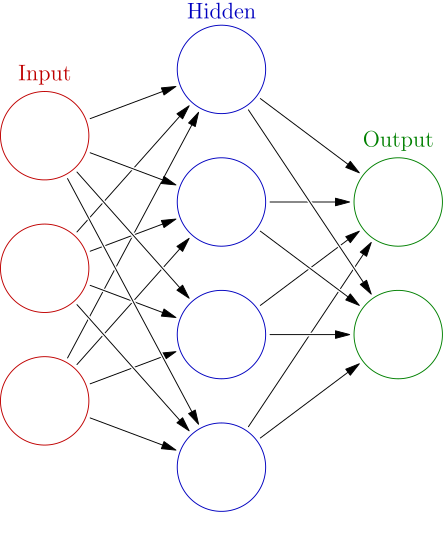
\includegraphics[width=0.25\textwidth]{nn_simple_1}~\caption{A simple Feed Forward Neural Network (FNN) with three layers: Input, Hidden and Output.\footnote{\cite{nn_simple_img_1}}}
        \label{fig:nn_simple_1}
    \end{figure}
    \noindent
    The Structure of a NN is also called Topology.
    \begin{mydef}{Neural Network Topology}
        The Topology of a Neural Network is its distinct arrangement of neurons, layers and the connections between the neurons.
        \label{definition:Topology}
    \end{mydef}
    \noindent
    For the neural network to perform functions, we also need to assign a weight to all the connections.
    This weight value ranges from -1 to 1 and can be thought of as the strength of a connection between neurons.
    \\
    In terms of computer science, this structure now resembles a directed, weighted graph, which is why we will call the neurons nodes and their connections edges from now on.
    \\ \\
    Now let's see, how information gets computed by a neural network by using the example of a computer vision NN, that recognizes digits on a black/white image:
    First, we need a way to encode the information into values for the nodes of the input layer, in our example the Brightness values of the single pixels.
    We assign these values to the nodes of the input layer.
    \\
    Then, for each node of the input layer, we look for all edges connected to that node.
    For each of these edges we multiply its weight by the value of the input node and add the result to the other node connected by the edge.
    \\
    After iterating through all the nodes of the one layer, we move the next layer.
    Now, the value of the nodes in this layer is the sum accumulated by the value of all connected nodes multiplied the weight of that connection:
    \begin{equation}
        v_x = \sum_{i=0}^{N}v_i * w_i\label{eq:sum_connected_nodes}
    \end{equation}
    Where:
    \textit{
        \begin{itemize}
            \item N is the number of connected nodes
            \item $v_x$ is the value of the current node
            \item $v_i$ is the value of the current node
            \item $w_i$ is the weight of the edge connecting the current node to node i
        \end{itemize}
    }
    \noindent
    Additionally, we can add a bias value $r_x$ ranging from -1 to 1 onto the value of the nodes.
    Afterward, an activation function is applied to the value of the nodes to fit the value of the node inside a preferred range.
    This activation function can also be thought of as the threshold of stimulation for a neuron to fire.
    Two examples for activation functions are:
    \begin{itemize}
        \item Sigmoid Function: $\sigma(x) = \frac{1}{1 + e^{-x}}$
        \item Rectified Linear Unit (ReLU): $\sigma(x) = \max{0, x}$
    \end{itemize}
    Plot of the activation functions:
    \\ \\
    \begin{center}
    \begin{tikzpicture}
     \begin{axis}[
     xmin=-6,
     xmax=6,
     ymin=0,
     ymax=6,
     ytick distance = 1,
     xtick distance = 1,
     minor tick num=1,
    axis lines = left,
    line width = 1.5pt,
    grid=both,
    major grid style={line width=0.8pt,draw=gray!50},
    minor grid style={line width=0.4pt,draw=gray!20},
    xlabel = \(x\),
    ylabel = {\(\sigma(x)\)}]
     \addplot[
        domain=-10:10,
        color=red,
        samples=1000.,
     ]{1/(1 + e^-x)};
\addlegendentry{\(Sigmoid\)}
     \addplot[
         domain=-10:10,
         color=blue,
         samples=1000.,
     ]{max(0,x)};
     \addlegendentry{\(ReLU\)}
     \end{axis}
    \end{tikzpicture}
    \end{center}
    \\ \\
    The final function for the value of one node is therefore:
    \begin{equation}
        v_x = \sigma\left(\sum_{i=0}^{N}v_i * w_i + r_x\right)\label{eq:value_node}
    \end{equation}
    Where (additionally to equation~\ref{eq:sum_connected_nodes}):
    \textit{
        \begin{itemize}
            \item $r_x$ is the bias of the node
            \item $\sigma$ is the activation function
        \end{itemize}
    }
    \noindent
    Now this value $v_x$ can be used in upcoming layers.
    When we reach the final layer after iterating through all the nodes and layers of the NN, we can read out its computed output.
    This output again is encoded in node values like the input and therefore needs to be decoded for the result.
    In the example of a digit detecting NN, we could encode the output with 10 output nodes, each representing one digit.
    The result could be decoded by using the output node with the highest value as result.
    This kind of output encoding, where all possible result get their own node is called One-hot encoding.
    With this kind of output encoding, the values of the output nodes can be interpreted as a certainty value for a specific result to be correct.
            \subsection{Remark: Functioning of NNs}\label{subsec:remark-about-the-funtioning-of-nns}
    Now that we have established how a NN works, it is important to understand why this kind of algorithm is revolutionary to computer science.
    \\ \\
    An algorithm is a set of functions applied in a certain order onto an input to receive a result.
    Traditionally, this algorithm was programmed with the help of mathematical operations, logic functions, loops, system functions and data structures, which are then converted into binary code for the processor.
    Of course, this also applies in the context of NNs, however, there is also a third layer of abstraction on top, which simulates the functioning of a brain with neurons.
    Since the traditional algorithm only enables the neurons in the NN, the third neuron-based layer is what computes the actual function of the NN\@.
    Therefore, NNs resemble more the functioning of a brain than a traditional algorithm.
    This difference results in implications for the functioning of an NN:
    Traditional algorithms represent actual mathematical calculations and are therefore deterministic.
    With NNs, the algorithm is based on different parameters for nodes and edges, which make it an unpredictable blackbox.
    Additionally, NNs don't represent actual functions but try to approximate them instead.
    This means it is hard to prove a neural network to be always accurate and is the reason why we often call the result of NNs its prediction.
            \subsection{An Example of NN learning: Backpropagation}\label{subsec:an-example-of-nn-learning:-backpropagation}
    We already know how a NN can make a prediction for a given input with the help of parameters, which encode for the structure and weights/biases of the NN.\@
    But how do we find such parameters for a given problem?
    The answer is to use machine learning, which trains the model to perform a certain task with the help of training data.
    \begin{mydef}{Machine Learning}
        Machine Learning is a subset of artificial intelligence that involves the use of algorithms and statistical techniques to optimize artificially intelligent models for a given problem.
    \end{mydef}
    One machine learning algorithm for NNs is called backpropagation, which is one of the simplest and most efficient ways to train a NN.\@
    \begin{mydef}{Backpropagation}
        The backpropagation algorithm is an algorithm that can optimize parameters for weights and biases of a NN within a fixed topology for a certain problem with the help of labeled data.
    \end{mydef}
    Backpropagation uses a training and test set containing unlabeled data for a problem.
    But what does a test set with unlabeled data mean in the context of machine learning?
    \begin{mydef}{(Un)labeled Data}
        Labeled data for a machine learning problem is a set of data with sample problems and the respective solutions.
        Unlabeled data instead only contains the sample problems.
    \end{mydef}
    The Machine Learning Process starts with an NN with fixed topology and random weights/biases.
    Then, you give the NN the training problems, whose predictions will be random at first.
    However, with the help of the corresponding solutions, you can refine the predictions of the NN by adjusting the parameters in a way that would let the NN make the correct prediction for the given problem.
    This is done by starting from the prediction of a certain problem its solution and propagating back through the whole NN until reaching the input layer.
    More specifically, you compute a cost function of
    The NN shouldn't be adapted only to a single problem but should be able to make accurate predictions for the whole training set as well as for unknown problems.
    To therefore prevent overcorrecting a NN for a single problem, we have to factor in a learning rate significantly smaller than 1 onto our correction.
    No we can train the NN on the whole training set for many generations, until the NN starts to make accurate predictions for the whole.
    To test the performance on unknown problems we can use a separate test set, which the NN wasn't trained on.

        \section{Evolutionary Computation (EC) \& Genetic Algorithms (GAs)}\label{sec:evolutionary-computation-(ec)-&-genetic-algorithms-(gas)}
    Now we will have a look at the Machine Learning Technique, this Thesis focuses on.
    Again, we will draw inspiration from Nature:
    \begin{mydef}{Evolutionary Computation}
    Evolutionary Computation (EC) is an Algorithm that optimizes a set of parameters for a problem with the help of natural selection.
    \end{mydef}
    One scenario for EC might be for example if you have a large set of data points of an unknown polynomial function with noise and outliers.
    If you want to find the underlying polynomial function, you could then employ Evolutionary Computation to find the best fitting parameters for such polynomial.
    So how do you find these parameters?
    \\ \\
    You start with an initial population of agents with a random set of parameters.
    For each generation of your population you will then repeat following steps:
    \begin{itemize}
        \item Fitness: First, you need to find out how good each agent (and its parameters) performs in the function they try to optimize for.
        The fitness evaluation can be done with an objective cost function or a competition between the agents, which evaluates their relative performances.
        In our example, the cost function might be the sum of the absolute differences between the data points and the output of the polynomial function.
        \item Selection: As a next step, you rank the agents performances to then pick the ones that have performed the best.
        \item Reproduction: The best agents pick is the part of the population that survives.
        These agents will then be replicated by copying their parameters (non-mating) of by merging parameters from different agents (crossover).
        \item Mutation: The agents parameters will then be mutated by either completely overwriting certain parameters with new random parameters or by shifting the existing parameters by a random number.
    \end{itemize}
    After a certain number of generations, you will then have the best performing set of parameters for a given problem.
    There is also one popular addition to EC, which draws inspiration from nature again:
    \begin{mydef}{Genetic Algorithm}
    A Genetic Algorithm (GA) is an implementation of EC that uses a genetic representation of the parameters.
    \end{mydef}
    Its main idea is to have genes that only encode indirectly for the parameters, and that can be on and off.
            \subsection{Gradient Descent \& Local Minima}\label{subsec:gradient-descent}
    We know from the previous Chapter(\ref{subsec:mutation}) that EC starts with an initial population of agents with random sets of parameters, which all have a cost determined by the cost function.
    Agents with relatively low cost survive the round and then get replicated a few times, mutated and again selected by cost.
    \\ \\
    This whole process strongly resembles a ball rolling down a hill in some terrain.
    On any given point on the terrain, de ball will roll down to the next neighboring point that is the lowest of all.
    Now, in EC the parameters for a function can be imagined as the horizontal coordinates for the ball meanwhile the cost of these parameters is the height at their location.
    The different mutations have parameters close to the original and can therefore be thought of as points close to the original in our terrain.
    And as the ball rolls down to the lowest of all neighboring points in any moment, EC again chooses the set of parameters with the lowest cost every cycle.
    This learning method is called Gradient Descent, as the algorithm evaluates all neighboring points and then follows this direction with the lowest cost and therefore steepest gradient.
    \\ \\
    So what does the ball example tell us about how EC learning works?
    Imagine a hill with each a shallow and a deep valley next to it.
    Depending on which side of the hill you place the ball in the beginning, it will roll in a different direction and end up in either of the two valleys with different height.
    From this we can take away following things about EC learning:
    \begin{itemize}
        \item (Minor) differences in the starting position can result in large differences in the end position and the respective cost.
        \item Once in reached a point with no downwards gradient, innovation halts for that agent, even if there is a lower cost point somewhere.
        Such points are called local minima.
    \end{itemize}
    The impact of starting position and local minima often pose a large problem for EC applications.
    Strategies to reduce the impact of such, are therefore essential for the Algorithms success.

        \section{Evolutionary Neural Networks (ENNs)}\label{sec:evolutionary-neural-networks-(enns)}
    After having covered all the basics about NNs and EC, we can now combine those concepts to create the algorithm, that this thesis is about.
    \begin{mydef}{Evolutionary Neural Networks}
        Evolutionary Neural Networks (ENNs) are Neural Networks that use Evolutionary Computation to optimize for its parameters for the NNs weights/biases and its topology.
    \end{mydef}
    ENNs are useful for complex machine learning problems and also work for unlabeled training data as long as there is a fitness function.
    Let's bring our knowledge about EC into the context of Neural Networks:
    The parameters ENNs encode for are for the weights, biases, nodes and edges of a Neural Network.
    You could either directly encode the NNs parameters as a graph or indirectly as genes, which would make it a Genetic Algorithm.
    ENNs still start with a random population of agents that are evaluated and selected by a fitness function.
    Then they are replicated (with crossover or non-mating) and finally mutated in following ways:
    \begin{enumerate}
        \item Change weights/biases: A new random value is set for the weight or bias of a random existing edge or node.
        \item Shift weights/biases: The value for an existing weight or bias of a random existing edge or node is altered by a random change but is kept close to the old value.
        \item Add edges: A new edge is added between two random unconnected nodes.
        \item Add nodes: A new node is added in between of a random existing edge.
        The old edge is removed and two new edges with random weight are added between the new node and the two other nodes each.
        \item Remove nodes/edges: A random node or edge in a way that doesn't cut off the input from the output layer.
    \end{{enumerate}}
    \section{Drawing Inspiration from the NEAT-Apporach}\label{sec:drawing-inspiration-from-the-neat-apporach}
        As already stated in the Thesis Statement(\ref{sec:thesis-statement}), Neuroevolution of Augmenting Topologies is a ENN machine learning algorithm by Kenneth O. Stanley and Risto Miikkulainen in 2002\footcite[p.105-106]{Neat_02}.
        One of its main innovations is that the initial population starts with NNs of lowest complexity and only increase topological complexity as its useful for the problem.
        In specific, you start with NNs that have only the nodes of the input layer connected to the nodes of the output layer.
        This should result in more efficient NNs for the problem, as the complexity is only increased when it improves the NNs performance.
        The NEAT algorithm therefore only needs the mutations 1. to 4. showed in the last chapter(\ref{sec:evolutionary-neural-networks-(enns)}) and doesn't need to remove complexity (mutation 5.)as it is already minimal.

    \section{Games}\label{sec:games}
    Let's also have a quick look at the games, this Thesis will train the ENNs on.
    \subsection{Simple Nim}\label{subsec:simple-nim}
    This game is a simplified version of Nim, where two players take turns removing an arbitrary amount of matches from a single stack with some number of matches.
    The player who removes the last match loses.
    Therefore, the winning strategy simply is to remove all matches from the stack but one, which forces the opponent to remove the last match, which makes them lose.
    \subsection{Nim}\label{subsec:nim}
    This game works similarly to Simple Nim (described in the last Section(\ref{subsec:simple-nim})) with the difference that there are multiple stacks with matches.
    Now, the player who removes the last match from the last unemptied stack loses.
    You can read up the winning strategy for Nim on Wikipedia\footcite{nim_23}.
    The winning strategy is much more complex, which forces the ENNs to learn a more complex strategy.
    \section{Related Work}\label{sec:related-work}
    The field of AI research in ENNs is largely studied and is often linked to games.
    In the following table, we can find some examples of ENN models that have been tested on games:

    \footnotesize
    \begin{center}
        \hspace*{-2cm}\begin{tabular}{|| l l l l l ||}
          \hline
          \makecell{\textbf{Author(s) \& Year}} &
          \makecell{\textbf{Model}} &
          \makecell{\textbf{Game/Benchmark}} &
          \makecell{\textbf{Computation}} &
          \makecell{\textbf{Accuracy}} \\
          \hline\hline
          \makecell{\cite{Neat_02}} &
          \makecell{NEAT} &
          \makecell{Double Pole Balancing\\With Velocities} &
          \makecell{3600\\evaluations} &
          \makecell{100\%} \\
          \hline
          \makecell{\cite{dama_22}} &
          \makecell{NEAT} &
          \makecell{Dama} &
          \makecell{$>$5000\\generations} &
          \makecell{81.25\%\\(wins against humans)} \\
          \hline
          \makecell{\cite{go_98}} &
          \makecell{SANE} &
          \makecell{Go} &
          \makecell{260\\generations} &
          \makecell{$>$75\%\\(vs Wally, 9$\times$9 board)} \\
          \hline
          \makecell{\cite{capture_02}} &
          \makecell{Custom\\ENN} &
          \makecell{Capture Game\\(subgame of Go)} &
          \makecell{100+\\generations\\(distributed)} &
          \makecell{No significant\\progress yet} \\
          \hline
          \makecell{\cite{backgammon_07}} &
          \makecell{Genetic\\ENN} &
          \makecell{Backgammon} &
          \makecell{256 pop,\\100–200\\generations} &
          \makecell{62.4\%\\(vs Pubeval)} \\
          \hline
        \end{tabular}\hspace*{-2cm}
    \end{center}
    \normalsize



    Note:
    Although the amount of fitness evaluation is a more accurate representation of computation load than the amount of generations, in many cases the amount of fitness evaluations isn't indicated and cannot be calculated.

    \chapter{Building my ENN}\label{ch:building-my-enn}

    \section{Algorithm Design}\label{sec:algorithm-design}
    Now, we will have a detailed look at how I used the concepts described in the last Chapter(\ref{ch:introduction}) to build an Evolutionary Neural Network that plays board games.
    First, I will explain the general Structure of my Code:
        \subsection{Overview}\label{subsec:overview}
    As already mentioned in the Thesis Statement(\ref{sec:thesis-statement}), this Project is written in the Rust Programming Language.
    If you don't understand the syntax of the code snippets, you can consult the online \("\)The Rust Programming Language\("\) booklet under: \url{https://doc.rust-lang.org/book/}
    \\ \\
    My Codebase is divided into different modules as well as a bin folder with main files, one of which has to be selected to be executed at the beginning.
    The other modules are divided into one module with the ENN algorithm, the other modules handle the different games, the ENNs learn to play.
    The ENN module is divided into two files:
    \begin{itemize}
        \item agent.rs: This file handles the NNs and the mutations on the NNs
        \item population.rs: This file handles the natural selection process and the data saving
    \end{itemize}
    The game modules provide the problems for the NNs handle the predictions of the NNs and finds the new game state after a move.
    It might also include an objective performance evaluation function to measure how well the NNs perform.
    I will now explain all the functions bottom up, starting with the Neural Network.
    I work with Rusts Structs which are similar to classes in other programming languages.
            \subsection{Neural Network}\label{subsec:neural-network}
    The struct \textit{NeurualNetwork} (defined in agents.rs) most importantly contains a two-dimensional vector of nodes, which encodes all the information of the NN\@:
    \begin{minted}{rust}
    pub struct NeuralNetwork {
        [...] // redundant side data about the NN
        pub nodes: Vec<Vec<Node>>,
    }
    \end{minted}
    The Vector inside (\mintinline{rust}{Vec<Node>}) represents a layer of the NN and the outside Vector (\mintinline{rust}{Vec<Vec<Node>>}) contains all layers of the NN\@.
    A \textit{Node} contains its bias and a vector for the incoming and outgoing edges:
    \begin{minted}{rust}
    pub struct Node {
        pub bias: f64,
        //edges stored in an adjacency list
        pub incoming_edges: Vec<Edge>,
        pub outgoing_edges: Vec<Edge>,
    }
    \end{minted}
    An \textit{Edge} contains the weight of the edge and its input/output node:
    \begin{minted}{rust}
    pub struct Edge {
        input: [usize; 2],
        out: [usize; 2],
        weight: f64,
    }
    \end{minted}
    The most important functions of the \textit{NeuralNetwork} struct are:
    \begin{itemize}
        \item \mintinline{rust}{new(input_nodes: usize, output_nodes: usize) -> Self {}}, which initializes the NN with all input and output nodes connected to each other with random weights and biases.
        \item \mintinline{rust}{predict(&self, input: Vec<f64>) -> Vec<f64>}, which computes the output of the NN for a given input with forward propagation algorithm described in the last Chapter(\ref{subsec:feed-forward-neural-networks-(fnns)}).
        \item \mintinline{rust}{new(input_nodes: usize, output_nodes: usize) -> Self {}}, which computes the neuron activation described in the last Chapter(\ref{subsec:feed-forward-neural-networks-(fnns)}).
        I use a variant of the \texit{ReLU} function, since the linearity for inputs above 0 of the ReLU function allows for more variety of neuron activation, which makes the NN more flexible and efficient.
        The variant I use is the \texit{ELU} function, which additionally tackles the problem of dead neurons in \texit{ReLU} by allowing for negative values.
        \item All mutation functions for the NN, which we will need in the next Subsection(\ref{subsec:mutation}).
    \end{itemize}
            \subsection{Mutation}\label{subsec:mutation}
    The mutation of the NNs is handled in the \textit{Agent} struct (defined in agent.rs), which includes a NN, its fitness and its Rank:
    \begin{minted}{rust}
    pub struct Agent {
        pub nn: NeuralNetwork,
        pub fitness: f64,
        pub rank: isize,
    }
    \end{minted}
    The function \mintinline{rust}{mutate(&mut self, mutations: usize) -> Self {} } has a number of mutations as a parameter which it applies to the NN of the Agent.
    For each mutation, it randomly selects one of the following mutations: Change weights/biases, Shift weights/biases, Add edges, Add nodes.
    All of these mutations have already been described in the last Chapter(\ref{sec:evolutionary-neural-networks-(enns)}), although there are some implementation details to mention:
    \begin{itemize}
        \item When inserting a new node between two connected nodes (mutation 4.), the inserted node will be added to a random layer in between the previously connected nodes.
        If the previously connected nodes are in neighboring layers, we create a new layer in between for the new node.
        %\item random selection details
        \item The shift mutation adds to the initial value a random float in the range 0.0 to 1.0 squared with random sign:
        $v_{new} = v_{old} + rand(-1, 1) * rand(0..1)^2$
        \item random weighted selection
    \end{itemize}

            \subsection{Evolutionary Computation}\label{subsec:natural-slection}
    The EC process starts with an initial population of Agents with new, minimal NNs created by the \mintinline{rust}{NeuralNetwork::new()} function (described in \ref{subsec:neural-network}).
    As we already established before (see~\ref{sec:evolutionary-computation-(ec)-&-genetic-algorithms-(gas)}), we now repeat the steps of performance evaluation, selection and mutation.
                \subsubsection{Competition and Fitness}
    In my case, the fitness evaluation works by letting the agents of a population compete against each other in the games.
    However, I can't let every agent play against all other agents, since the needed time increases quadratically with population size.
    My solution therefore is to use my circular Pairing algorithm.
    This algorithm, I first define a number of opponents each agent needs to play against.
    For each of those games, I generate a new distance, where I now loop through my list of agents and pair agent i with agent i + distance.
    I also check before, that the distance isn't a multiple of any distance we had previously, since this would result in the same agents being paired twice.
    \\ \\
    Now, we need to evaluate the fitness of the agents with the fitness function.
    The main idea for the fitness function is to simply count the number of wins an agents has made during the competition.
    Of course, there are other possibilities to evaluate the performance of the agents that may represent an agents performance more accurately.
    The reason why I still first try to use the number of wins as fitness is because it is a generally applicable function to any game.
    Counting the number of wins doesn't require a deeper understanding of the game, which is very useful in games that are indeterministic.
    This also enables the ENNs to find their own new strategy for the game, which is finally the goal of AI training.
                \subsubsection{Natural Selection}
    After the fitness evaluation, we now can test the performance of the generation (in the next section~\ref{subsec:performance-tests}) and then generate the new population.
    The new population is made up by some portion of each of following:
    \begin{itemize}
        \item Agents from the last generation:
        The main part of the new population will be drawn from agents from the old generation with high fitness.
        This works by drawing all needed agents randomly with the probability of an agent being drawn being its fitness.
        We can also raise the fitness to some power to either allow more or less survival of non top-performing agents.
        \item Random agents from the last generation:
        Some fraction of the new population is made up of randomly selected agents from the last generation, which might help counter a population with the top performing agents stuck in local minimum.
        \item New random agents:
        Another fraction of the new population is made up of newly generated random agents, which might help counter overly complex NNs and also local minima in a population.
    \end{itemize}
    Now that we have generated our new population, we can start over the whole process.
            \subsection{ENN Parameters}\label{subsec:enn-parameters}
    As already mentioned in the Thesis Statement(\ref{sec:thesis-statement}), my research involves testing my implementation with several configurations of different parameters and then evaluate their performance with the stats described in the following section(\ref{subsec:performance-tests}).
    Here is a list of all possible parameters influencing my ENNs:
    \begin{itemize}
        \item General: Size of the population
        \item Game: Initial state of the game, game function that decodes the NN prediction and executes the move on the current state
        \item Competition: Number of opponents per agent
        \item Selection: Fitness exponent, share of old best agents, random agents from last generation and new random agents making up the new population besides agents selected by fitness
        \item Mutation: Min and max amount of mutations per agent, weight/probability of the different mutations
        \item Evaluation: Number of games from the best agent against old best agents
    \end{itemize}
    For each test, we then save a file with the information about the value of all these parameters.

    \subsection{Performance Tests}\label{subsec:performance-tests}
    To see how the Agents perform in the games, we need to track some stats and games.
    We save following data every generation after the competition phase:
    \begin{itemize}
        \item The fitness of the best agent: This stat shows us, how much better the best agent performs relatively to the average agent
        \item Wins against older generation: We pair the best agent against an evenly distributed set of the best agents from past generations to track relative performance to the past.
        As long as this number is above 50\%, we should expect improvement over older generations.
        \item Objective grading: This stat is the performance evaluation of the best agent based on some algorithm that either plays mathematically perfect or (in non-deterministic games) is generally accepted to play well.
        It is important to note that we primarily don't use this algorithm for the fitness function, because of the points previously mentioned in section~\ref{subsec:natural-slection}.
        \item Number of turns: We track the average number of turns the agents needed while playing their competition games.
        In Nim, low turn count generally means better play.
        \item Average amount of hidden layers and nodes per hidden layer: We track these stats to see how complex the topologies of our NNs in the population are.
        \item Best agent layer sizes and edges: We track these topological stats to see how complex the best solution is.
        \item Best agent games: We track the whole game turn for turn played by the best agent from the current generation against each the best agent from the last generation and a randomly selected best agent from previous generations.
        With this game logs, we can see what moves our agents make in real games and try to grasp their tactics and strategies.
    \end{itemize}
            \subsection{Nim}\label{subsec:nim-implementation}
    For the nim game, I implemented a few different game modes as well as objectively perfectly playing dynamic programming algorithm.
    Let's first look at the general idea of how a game is played.
                \subsubsection{General Approach}
    Each game starts with a first game state, which is derived from the initial state parameter.
    A game state is a list where the length is the amount of stacks in that game and each value $v_i$ stands for the amount of matches on the i-th stack.
    Then, the competing agents take turns playing their moves.
    In one turn, the agent whose turn it is, reads the current game state as input and then makes a prediction for its move.
    A move indicates the stack where the matches are removed as well as the number of removed matches.
    Then the game computes the new game state after the move or ends the game if all stacks are empty.

                \subsubsection{Encoding and Decoding}
    Our input is directly encoded into the input layer of the NNs, which means the input layer has the same size as the state.
    The values of the input nodes are directly copied from the game state list and therefore also represent the amount of matches on the i-th stack.
    \\ \\
    For the output, I implemented two different ways of encoding.
    \begin{itemize}
        \item Direct encoding: We have two output nodes where the value for the first represents the index of the stack and the second value represents the amount of matches that are removed.
        \item One-hot encoding: The first $N$ output nodes encode for the index and the following nodes encode for the amount of matches removed.
        For both the nodes encoding for index and amount the node with the highest value is finally used as output.
        The output layer therefore has length $l = N + \max(state_{initial})$, where $N$ is the amount of stacks and $\max(state_{initial})$ is the highest possible amount of matches on a stack.
    \end{itemize}
    Direct encoding is the more straight forward approach with lower NN topology whereas one-hot encoding ensures that the output stays in a reasonable range.
                \subsubsection{Game Modes}
    There are game modes \texit{Simple Nim} and \texit{Nim} with some configuration possibilities:
    \\
    In \texit{Nim}, each stack of the initial state can hold matches whereas in \textit{Simple Nim}, the value of all stacks but one randomly chosen stack is set to 0.
    \\
    The stack sizes in the initial state equal the corresponding value from the initial state list parameter except for the configuration \textit{random}, where the stack sizes of the initial state are randomly selected with the corresponding value in the initial state list parameter as upper bound.
    \\
    Another configuration involves the output decoding.
    With strict grading, illegal moves lead to a game loss, whereas in safe grading, the closest legal move to the illegal prediction is played.
                \subsubsection{Objective Grading}
    To have an exact measure of performance, I implemented a Dynamic Programming (DP) algorithm that knows the best moves for each given state.
    It works by first defining a base case, which in case of Nim is every stack being empty and the result a loss.
    Then, it starts with the initial state and tries out all possible moves using recursion.
    For each state it tries to find a move that forces the opponent into a losing position.
    If it can find such move, the position is winning, but if all moves lead to winning position for the opponent, the algorithm returns the position with the highest minimum moves for the opponent to win.
    It also stores the result for each already computed state, so that all other paths that lead to that position can use the precomputed result.
    \\ \\
    Now, that we know for all positions if they're winning, we can use this to grade moves of our agents:
    For each move, an agent gets one point if
    \begin{itemize}
        \item the agent had a winning state and made a move that got the opponent into a losing state,
    \end{itemize}
    or if
    \begin{itemize}
        \item the agent had a losing state and made a move that required the maximal amount of moves for the opponent to win.
    \end{itemize}
    The sum of all points an agent has collected is then divided by the amount of moves it has made to get the final performance score.

    \section{First Findings}\label{sec:first-findings}
    Now we can test our ENN algorithm with the games and different parameters.
    The general approach is to start by training the ENNs on easy problems whilst observing the effect of different parameters on the result.
    We therefore start with the game Simple Nim.
            \subsection{Simple Nim}\label{subsec:simple-nim-results}

    \subsection{Nim}
        \section{Complexification}
    \chapter{Wrapping Up}
        \section{Auto Review}
        \section{Future Work}
    \chapter{Appendix}
        \section{Code}
        \section{Data}
        \section{Documentation}
        \section{References}
    \printbibliography

\end{document}
